\section{Zielsetzung}
In diesem Experiment wird mithilfe einer Ultraschallsonde unter Verwendung des Doppler-Effektes die Fließgeschwindigkeit einer Flüssigkeit in einem Rohr bestimmt. Weiterhin wird auch das Strömungsprofil innerhalb des Rohres aufgezeichnet.
\section{Theorie}
Schall kann anhand seiner jeweiligen Frequenz in verschiedene Bereiche kategorisiert kategorisiert werden. Menschen hören Frequenzen zwischen $16$ und $20$ kHz. Die Frequenzen unterhalb dieser Schwelle werden als Infraschall, die oberhalb bis zu einem Grenzwert von $1$ GHz als Ultraschall bezeichnet. Oberhalb dieses Grenzwertes wird von Hyperschall gesprochen. \\
Wenn sich eine Schallquelle relativ zu ihrem Beobachter in Bewegung befindet, tritt eine Frequenzverschiebung auf. Dieses Phänomen wird als Doppler-Effekt bezeichnet. Wenn sich eine Schallquelle der Frequenz $f_0$ mit der Geschwindigkeit $v$ auf einen ruhenden Beobachter zubewegt, erhöht sich die beobachtete Frequenz zu $f_{gr}$, während die Frequenz im umgekehrten Fall einer sich entfernenden Quelle zur kleineren Frequenz $f_{kl}$ hin verschoben wird. Die jeweils verschobene Frequenz kann mithilfe der Formel
\begin{equation}
f_{gr/kl}=\frac{f_0}{1 \mp \frac{v}{c}}
\end{equation}
berechnet werden, wobei die Konstante $c$ die Schallgeschwindigkeit bezeichnet. \\
Wenn sich wiederum der Beobachter mit der Geschwindigkeit $v$ auf eine ruhende Quelle zubewegt, wird die Frequenz zum höheren Wert $f_h$ verschoben. Ein sich entfernender Beobachter resultiert somit wieder in einer geringeren Frequenz $f_n$. Diese Verschiebung wird durch die Gleichung 
\begin{equation}
f_{h/n}=f_0(1 \pm \frac{v}{c})
\end{equation}
beschrieben. \\
Wenn Schall auf eine bewegtes Objekt trifft, wird gemäß dem Doppler-Effekt die Frequenz verschoben, sodass die Verschiebung Rückschlüsse auf die Geschwindigkeit des Objektes zulässt. Dies kann beispielsweise verwendet werden, um die Fließgeschwindigkeit von Blut zu bestimmen. Die Differenz der gemessenen zur ursprünglichen Frequenz $f_0$ wird allgemein durch die Formel 
\begin{equation}
\Delta f=f_0\frac{v}{c}(\cos(\alpha)+\cos(\beta))
\end{equation}
beschrieben, wobei $\alpha$ bzw. $\beta$ den Winkel zwischen dem Geschwindigkeitsvektor $v$ und der Wellennormale der ein- oder auslaufenden Welle beschreibt. In diesem Falle wird das Impuls-Echo Verfahren verwendet, bei dem der Ultraschallsender simultan als Empfänger fungiert, weshalb die Winkel von ein- und auslaufender Welle übereinstimmen ($\alpha=\beta$), wie in Abbildung \ref{fig:Dopplersonographie} dargestellt. Daraus ergibt sich für die Frequenzverschiebung:
\begin{equation}
\Delta f=2f_0 \frac{v}{c}\cos(\alpha).
\end{equation} 
\begin{figure} [h]
    \centering
    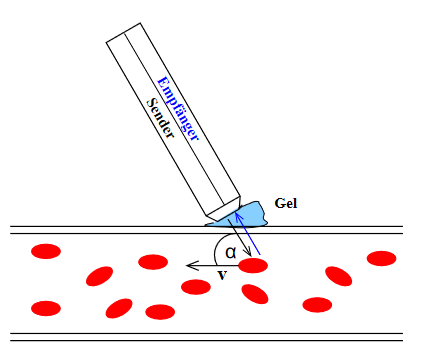
\includegraphics[width=6cm, keepaspectratio]{Dopplersonographie Skizze}
    \label{fig:Dopplersonographie}
    \caption{Schematische Darstellung der Dopplersonographie mit dem Impuls-Echo Verfahren}
 \end{figure} 
Bei der Erzeugung von Ultraschallwellen bedient man sich des sogenannten reziproken piezoelektrischen Effektes. Wenn ein piezoelektrischer Kristall (wie z.B. Quarz) entlang seiner polaren Achse in einem elektrischen Wechselfeld platziert wird, wird dieser zu Schwingungen angeregt, was zur Emission von Ultraschallwellen führt. Umgekehrt kann ein solcher Kristall auch als Empfänger verwendet werden, der Schallwellen registriert, da er von diesen zu Schwingungen angeregt wird. \\
